\documentclass[runningheads]{llncs}
\usepackage{amssymb}
\usepackage{tikz}
\usepackage{amsmath}
\usepackage{xcolor}

\begin{document}

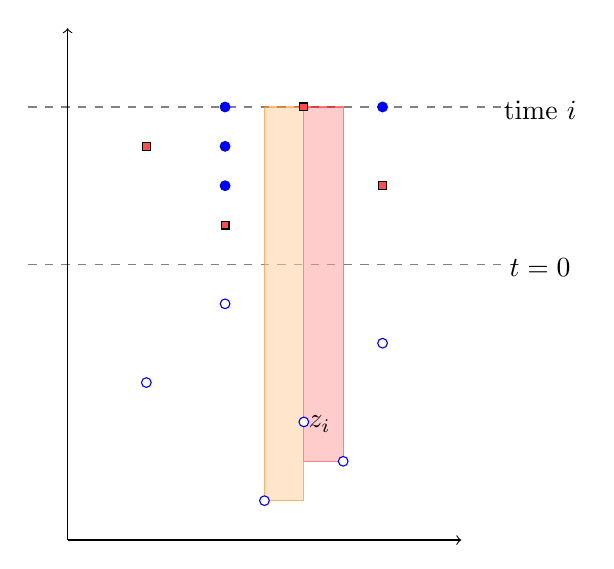
\begin{tikzpicture}[scale=.5]
\draw [gray,dashed] (-1,0)--(11,0) ;
\draw [gray,dashed] (-1,4)--(11,4) ;
\draw[->][black] (0,-7) -- (10,-7);
\draw[->][black] (0,-7) -- (0,6);

\filldraw[red!40!white,opacity=.5,draw=red] (6,4) rectangle (7,-5);
\filldraw[orange!40!white,opacity=.5,draw=orange] (6,4) rectangle (5,-6);

\filldraw[draw=black,fill=red!70!white] (3.9,0.9) rectangle (4.1,1.1) (7.9,1.9) rectangle (8.1,2.1) (1.9,2.9) rectangle (2.1,3.1) (5.9,3.9) rectangle (6.1,4.1) ;

\filldraw[blue] (4,2) circle (3.5pt) (4,3) circle (3.5pt) (4,4) circle (3.5pt) (8,4) circle (3.5pt)  ;

\filldraw[draw=blue, fill=white] (4,-1) circle (3.5pt) (8,-2) circle (3.5pt) (2,-3) circle (3.5pt) (6,-4) circle (3.5pt) (7,-5) circle (3.5pt) (5,-6) circle (3.5pt);

\draw[black](12,0.4)node[anchor=north]{$t=0$};
\draw[black](12,4.4)node[anchor=north]{time $i$};
\draw[black] (6.4,-3.6)node[anchor=north]{$z_i$} ;
\end{tikzpicture}

\end{document}